\lez{6}{12-03-2020}{}
Procediamo con il conto della scorsa lezione assumendo l'equilibrio radiativo nella nostra atmosfera, ovvero l'assenza di sorgenti e di pozzi in quest'ultima. In questo modo il flusso che arriva al nostro strato dalle profondità dell'atmosfera è conservato e passa oltre, quindi:
\[
	\frac{\partial F}{\partial \tau } = 0 
.\] 
In questo modo si ricava dalla \ref{eq:flux_0} che:
 \[
	J = s
.\] 
Quindi l'equazione del trasporto (\ref{eq:trasport-parallel-plane}) diventa:
\begin{align}
	\mu \frac{\mbox{d} I}{\mbox{d} \tau } =& - J + I =\\
	= & I - \frac{1}{2}\int_{-1}^{1} I( \tau )  d\mu  
.\end{align}
Quest'ultima è una equazione integro-differenziale in $I$, si risolve con dei metodi analitici particolari che vanno fuori dalla portata del corso.\\
Vediamo allora se studiandone i momenti possiamo far in modo di trovare una soluzione, seppur restringendo ancora il campo della soluzione. Partiamo dal momento di ordine 1:
\begin{align}
	&\frac{\mbox{d} P}{\mbox{d} \tau } = \frac{F}{c} &
	&\ce{ ->[Integro]}
	& P( \tau ) = \frac{F}{c}\left( \tau + q \right) 
.\end{align}
Dove $q$ è una costante di integrazione. Vedremo che trovare questa costante ci permetterà di risolvere l'atmosfera.\\ 
Abbiamo visto che in caso di LTE e considerando solo la prima correzione alla legge di Kirchhoff continua ad esser valido che:
\[
	P = \frac{u}{3}
.\] 
Questa abbiamo detto esser valida fintanto che il contributo anisotropo è piccolo rispetto a quello isotropo, quindi valido finchè non ci spostiamo verso strati esterni della atmosfera, tali che $T < T_{\text{eff}}$. Per proseguire con il conto analitico noi facciamo un'altra approssimazione:
\begin{defn}[Approssimazione di Eddington]{def:Approssimazione di Eddington}
	La relazione $P = u /3$ resta valida in tutta l'atmosfera, nonostante la possibile anisotropia.
\end{defn}
Possiamo quindi riassumere tutte le semplificazioni in cui ci siamo posti:
\begin{enumerate}
	\item Atmosfera a piani paralleli
	\item LTE (con correzione anisotropa)
	\item Atmosfera grigia
	\item Equilibrio radiativo
	\item Approssimazione di Eddington
\end{enumerate}
Grazie alla quinta è possibile inoltre affermare che resta vero in tutta l'atmosfera:
\[
	u = \frac{4\pi}{c}J
.\] 
E inoltre vale sempre che $J = s$.\\
Con questa nuova approssimazione possiamo mostrare la dipendenza di $s$ da $q$, infatti usando le ultime due relazioni si ha che:
\[
	P = \frac{4\pi J}{3c} = \frac{4\pi s}{3c} = \frac{F}{c}\left( \tau + q \right) 
.\] 
Quindi:
\[
	s( \tau )  = \frac{3F}{4\pi}\left( \tau + q \right) 
.\] 
Possiamo sfruttare questa espressione per la $s$ all'interno della soluzione che abbiamo trovato per $I_{\nu} $ nel caso di raggi uscenti dall'atmosfera ($0 \le \mu  \le 1$):
\[
	I( \tau , \mu )  = - \int_{\infty}^{\tau } \frac{s( \tau ') }{\mu } \exp\left(- \frac{\tau ' - \tau }{\mu } \right) d\tau ' 
.\]
Supponiamo di voler calcolare la brillanza nel punto più esterno alla nostra atmosfera, ovvero quello con $\tau = 0$, in tal caso avremo:
\[
	I( 0 , \mu )  = -  \int_{\infty}^{0 } \frac{s( \tau ') }{\mu } \exp\left(- \frac{\tau ' }{\mu } \right) d\tau ' 
.\] 
E sostituendo a questo punto la nostra $s$: 
\begin{align}
	I( 0, \mu ) =& - \int_{\infty}^{0} \frac{3F}{4\pi}\left( \tau ' + q \right) \exp\left( - \frac{\tau '}{\mu } \right)  d\tau '=\\
	=& - \frac{3F}{4\pi}
	\left[ \int_{\infty}^{0} \tau ' \exp\left( - \frac{\tau '}{\mu } \right) \frac{d\tau '}{\mu } + 
	q \int_{\infty}^{0} \exp\left( -\frac{\tau '}{\mu } \right) \frac{d\tau '}{\mu }  \right] =\\
	= &  \frac{3F}{4\pi}\left( \mu + q \right) 
.\end{align}
Un trucchetto che possiamo fare adesso è quello di trovare $F_{\text{out}}$ (uscente) in funzione di $I$, vedremo che facendo ciò il flusso si semplifichera permettendoci di ricavare $q$:
\begin{align}
	F_{\text{out}} =& 2\pi \int_{-1}^{1} I \mu d\mu = \\
	= & 2\pi \int_{-1}^{1} \frac{3F}{4\pi}\left( \mu + q \right) \mu d\mu = \frac{3F}{2}\left[ \int_{0}^{1} \mu ^2d\mu + \int_{0}^{1} \mu d\mu    \right] =\\
	= &\frac{3F_{\text{out}}}{2}\left[ \frac{1}{3} + \frac{q}{2} \right] 
.\end{align}
Quindi semplificando il flusso si ha:
\[
	q = \frac{2}{3}
.\] 
E inserendolo in $s( \tau ) $ e in $I_{\nu} ( 0, \mu ) $:
\[
	s( \tau ) = \frac{3F}{4\pi}\left( \tau + \frac{2}{3} \right) \quad \quad \quad I( 0, \mu ) = \frac{3F}{4\pi}\left( \mu + \frac{2}{3} \right) 
.\] 
Con queste informazioni possiamo per la prima volta trovare il profilo di temperatura per la nostra stella:
\[
	s = \frac{c}{4\pi} u = \frac{3F}{\pi}\left( \tau  + \frac{2}{3}\right) \implies cu = 3F\left( \tau + \frac{2}{3} \right) 
.\]
Ricordando che in LTE si ha anche $u = aT^{4}$, $F = \sigma  T^{4}$:
\[
	caT^{4}=3\sigma T_{\text{eff}}^{4}\left( \tau +\frac{2}{3} \right) \implies \left( T( \tau ) \right) ^{4}= \frac{3}{4}T^{4}_{\text{eff}}\left( \tau +\frac{2}{3} \right)  
.\] 
Notiamo nel nostro profilo che la temperatura efficace si ha per $\tau  = \frac{2}{3}$.\\
\subsection{Limb Darkening}%
Possiamo inoltre osservare un altro fenomeno interessante, infatti si ha che, all'aumentare dell'inclinazione $\mu $ diminuisce l'intensità uscente $I( 0, \mu ) $, questo da luogo al fatto che, per una sorgente che possiamo risolvere otticamente, la zona più interna risulterà più brillante della zona esterna.\\
Per convincerci del fatto che vi è un fenomeno del genere possiamo ragionare in termini di cammino libero medio $\tau $:
\begin{figure}[H]
    %This is a custom LaTeX template!
    \centering
    \incfig{fenomeno-di-limb-darkening}
    \caption{\scriptsize Fenomeno di Limb Darkening}
    \label{fig:fenomeno-di-limb-darkening}
\end{figure}
\noindent
Abbiamo visto che i fotoni che riescono ad emergere hanno cammino libero medio unitario, quindi hanno anche $\tau = 1$. \\
Ponendo un osservatore a sinistra in Figura \ref{fig:fenomeno-di-limb-darkening} possiamo notare che, andando verso l'esterno del disco la condizione $\tau =1$ è rispettata in zone sempre più superficiali. Se abbiamo che vale (quasi) la fisica del corpo nero per la stella e se la temperatura aumenta verso l'interno questo significa che raggi più profondi hanno anche intensità maggiore, quindi il centro del disco sarà più luminoso. Ecco spiegato il fenomeno del Limb Darkening in modo intuitivo.\\
Possiamo vedere questo effetto nel sole:
\begin{figure}[H]
	\centering
	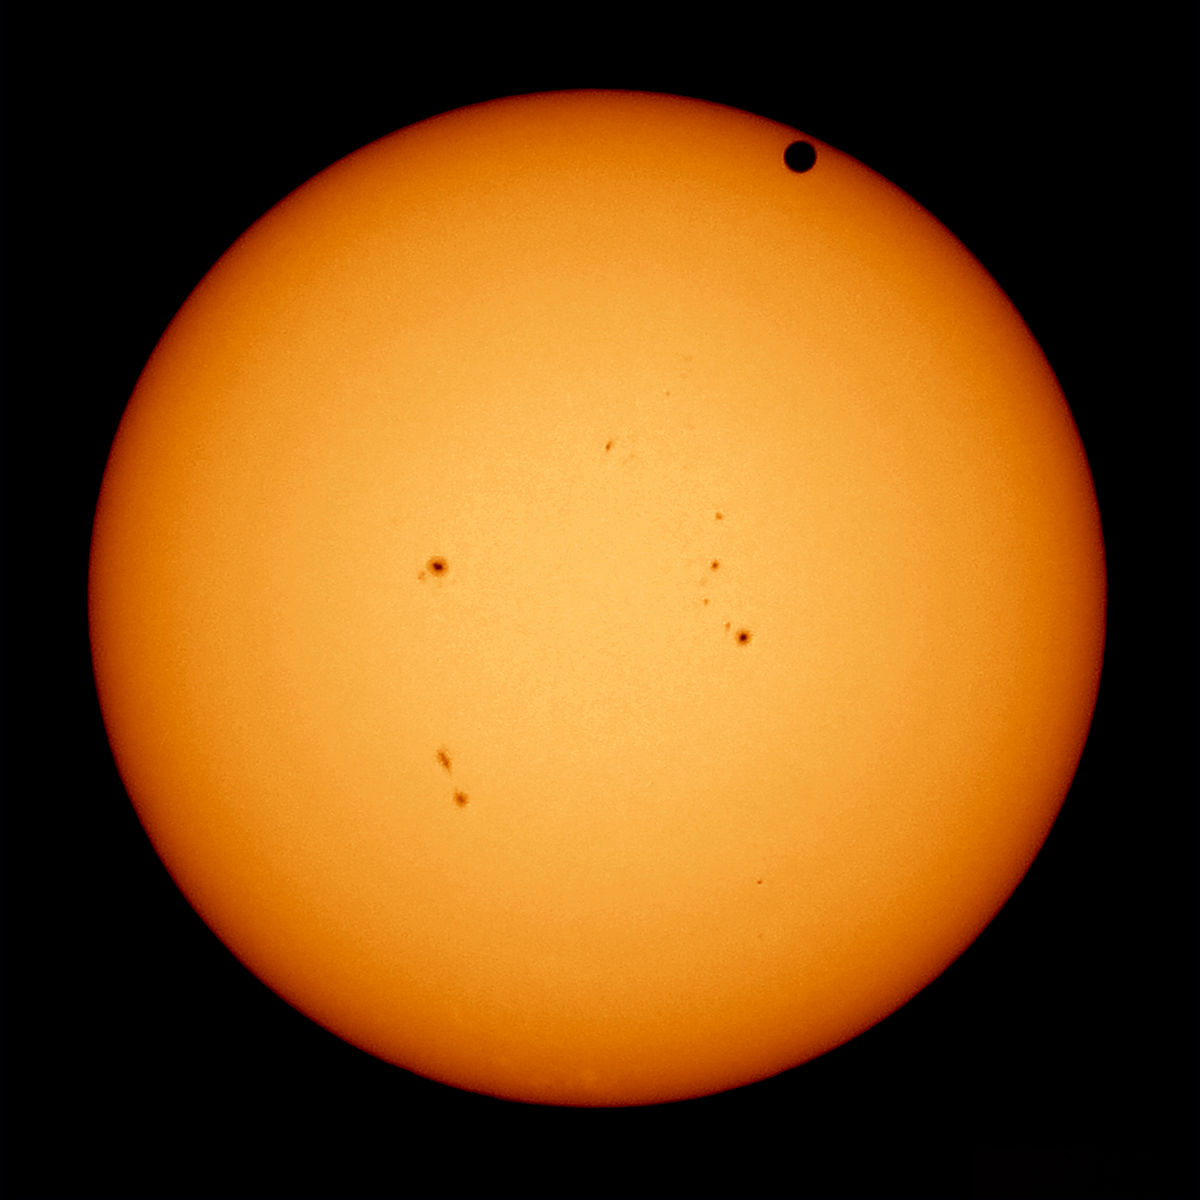
\includegraphics[width=0.6\textwidth]{figures/Limb.jpg}
	\caption{Limb Darkening nel disco del sole.}
	\label{fig:figures-Limb-jpg}
\end{figure}
\noindent
In cui con le stesse motivazioni (corpo nero ) si può spiegare anche l'effetto cromatico che, andando verso l'esterno si passa da giallo a rosso.\\
Concludiamo valutando l'intensità al centro su quella al bordo:
\[
	\frac{I( 0,0) }{I( 0,1) } = \frac{2F / 4\pi}{5F / 4\pi} = \frac{2}{5} 
.\] 
A conferma di quanto detto finora.
\subsection{Righe nello spettro stellare}%
Possiamo adesso spiegare  perchè nello spettro solare si possono trovare delle righe di assorbimento osservando dalla terra, abbandoniamo il modello di atmosfera grigia e torniamo a considerare le frequenze:
\[
	\mu \frac{\mbox{d} I_{\nu} }{\mbox{d} \tau _{\nu} } = -s_{\nu} + I_{\nu} 
.\]
I momenti della equazione sono gli stessi di prima, soltanto che adesso son monocromatici. Manteniamo l'ipotesi di equilibrio radiativo $F = cost$, considerando però il fatto che questo non significa che il flusso monocromatico $F_{\nu} $ sia costante, solo che il totale è conservato.
Quindi abbiam oche il flusso totale resta costante ma sarà ridistribuito tra le varie frequenze. \\
La radiazione che emerge dalla superficie può essere (qualitativamente) corretta con il primo ordine:
\[
	I_{\nu} ( 0, \mu ) \approx B_{\nu} ( 0) + \mu \frac{\mbox{d} B_{\nu} }{\mbox{d} \tau _{\nu} } 
.\] 
Concentriamoci sulla radiazione proveniente dal centro del disco $\mu = 1$:
\[
	I_{\nu} ( 0, 1) \approx B_{\nu} ( 0) +\frac{\mbox{d} B_{\nu} }{\mbox{d} \tau _{\nu} } \approx B_{\nu} ( \tau _{\nu} = 1) 
.\] 
Abbiamo ottenuto un risultato congruo con quanto visto sopra per il Darkening: dal centro del disco ci arrivano principalmente fotoni che si sono formati a  $\tau _{\nu} = 1$, infatti ci arriva una radiazione di corpo nero corrispondente a $B_{\nu} ( \tau _{\nu} = 1) $.\\
Prendiamo adesso un coefficiente di assorbimento fatto in questo modo: 
\begin{figure}[H]
    %This is a custom LaTeX template!
    \centering
    \incfig{coefficiente-di-assorbimento-per-una-riga}
    \caption{\scriptsize Coefficiente di assorbimento per una riga}
    \label{fig:coefficiente-di-assorbimento-per-una-riga}
\end{figure}
\noindent
Con questo coefficiente di assorbimento ci aspettiamo una riga, infatti abbiamo visto che il coefficiente di assorbimento ha le dimensioni di un inverso di un a lunghezza, abbiamo anche visto che questo decreta il cammino libero medio dei fotoni a tale frequenza $l_{\nu} $:
\[
	\alpha _{0} > \alpha _{c}
.\] 
\[
	l_{0} = \frac{1}{\alpha _{0}} < l_{c} = \frac{1}{\alpha _{c}}
.\] 
Quindi il cammino libero medio nell'intevallo di frequenze della riga sarà minore di quello nel continuo, questo spiega il motivo della presenza di righe di assorbimento. Infatti nella atmosfera stellare abbiamo visto essere presente un gradiente di temperatura (la temperatura aumenta andando verso l'interno), i fotoni che formano il continuo provengono da zone più profonde della atmosfera (in cui la temperatura è $T_{c}$), quelli della riga da zone più superficiali (in cui vi è $T_{0}$).
\[
	T_{0} < T_{c}
.\] 
Quindi se è vero che l'intensità proveniente dalla stella segue un andamento tipico di un corpo nero alla profondita ottica $\tau_{\nu} = 1$ ed è anche vero che le curve $B( \tau _{\nu} ) $ non si intersecano mai: 
\[
	I_{0} \approx B_{0}( T_{0}) <  I_{c} \approx B_{c}( T_{c}) 
.\] 
\begin{figure}[H]
    %This is a custom LaTeX template!
    \centering
    \incfig{riga-di-assorbimento}
    \caption{\scriptsize Riga di assorbimento}
    \label{fig:riga-di-assorbimento}
\end{figure}
\noindent
Quindi vediamo una intensità minore per le frequenze in cui $\alpha _{\nu} $ è "alto", viceversa sono più intense le frequenze per cui $\alpha _{\nu} $ è basso. Per questo motivo vediamo delle righe di assorbimento.
